\documentclass[11pt]{book} % or report
\usepackage[utf8]{inputenc}
\usepackage{amsmath}
\usepackage{amsfonts}
\usepackage{amssymb}
\usepackage{geometry}
\geometry{a4paper, margin=1in}
\usepackage{graphicx}
\usepackage[hidelinks]{hyperref}
\usepackage{amsthm}
\usepackage{tikz}
\usepackage{subcaption}
\usetikzlibrary{positioning}
\usepackage{pgfplots} % Add this line to import the pgfplots package


\newtheorem{theorem}{Theorem}[section]
\newtheorem{definition}{Definition}[section]
\newtheorem{corollary}{Corollary}[section]
\newtheorem{claim}{claim}[section]


\title{Summary of 76909 - Neural Learning}
\author{Hadar Tal}
\date{Winter 2024}

\begin{document}

\frontmatter
\maketitle
\tableofcontents

\mainmatter
\chapter{Mathematical Background}

\section{Math notations}

In this course, we adopt standard mathematical notations to maintain clarity and consistency. Scalars are denoted by lowercase or uppercase italic letters (e.g., \(a\), \(A\)), vectors by lowercase bold letters (e.g., \(\mathbf{v}\)), and matrices by uppercase bold letters (e.g., \(\mathbf{M}\)). The set of real numbers is represented by \(\mathbb{R}\), and \(\mathbb{R}^n\) denotes an \(n\)-dimensional vector space. Functions are represented as \(f(\cdot)\), and derivatives are denoted using the prime notation (e.g., \(f'(x)\)) or the \(\nabla\) symbol for gradients.

The gradient of a function with respect to a variable, denoted as \(\frac{df}{dx}\), represents the rate of change of the function \(f\) with respect to the variable \(x\). This notation is predominantly used in the context of single-variable functions. In the realm of multivariable functions, the gradient is a vector of all partial derivatives, indicating the direction and rate of the steepest ascent in the function's value. The gradient is represented as \(\nabla f\) or \(\vec{\nabla} f\), where each component of the vector \(\nabla f = \left(\frac{\partial f}{\partial x_1}, \frac{\partial f}{\partial x_2}, \ldots, \frac{\partial f}{\partial x_n}\right)\) signifies the partial derivative of \(f\) with respect to each variable \(x_i\).

The directional gradient, on the other hand, gives the rate of change of the function in a specific direction, represented by a unit vector \(\mathbf{u}\). It is calculated as the dot product of the gradient and the direction vector, denoted by \(\nabla_{\mathbf{u}} f = \nabla f \cdot \mathbf{u}\). This quantity measures how fast the function changes at a point in a given direction.

The delta symbol (\(\Delta\)), often used to signify change or difference, is employed in various contexts in mathematics and physics. For instance, \(\Delta x\) represents a change in the variable \(x\), and \(\Delta f(x) = f(x_2) - f(x_1)\) denotes the change in the function \(f\) as the argument moves from \(x_1\) to \(x_2\). This notation is essential for describing finite differences, differences in quantities, and is fundamental to the concepts of differentiation and integration.


\section{Vector and matrix derivatives of scalar functions}

\subsection{Definitions}

The derivative of a scalar function with respect to a vector, \(\nabla_{\mathbf{x}} f\), results in a vector of partial derivatives. Similarly, the derivative of a scalar function with respect to a matrix, \(\nabla_{\mathbf{X}} f\), yields a matrix where each element is the partial derivative of \(f\) with respect to the corresponding element in \(\mathbf{X}\).

\subsection{Examples}

For a function \(f(\mathbf{x}) = \mathbf{x}^T\mathbf{A}\mathbf{x} + \mathbf{b}^T\mathbf{x} + c\), where \(\mathbf{x}\) is a vector, \(\mathbf{A}\) is a matrix, \(\mathbf{b}\) is a vector, and \(c\) is a scalar, the gradient with respect to \(\mathbf{x}\) is \(\nabla_{\mathbf{x}} f(\mathbf{x}) = 2\mathbf{A}\mathbf{x} + \mathbf{b}\).

\subsection{multi-variate chain rule}
Let $y(x,z)$ be a function of $x$ and $z$, and $x(w)$ and $z(w)$ be functions of $w$. 
Then the derivative of $y$ with respect to $w$ is given by:
\begin{equation}
    \frac{dy}{dw} = \frac{\partial y}{\partial x} \frac{dx}{dw} + \frac{\partial y}{\partial z} \frac{dz}{dw}
\end{equation}

%
%
%

\section{Probability}

\subsection{Definitions}

Probability theory provides a mathematical framework for quantifying uncertainty. A probability space is defined by a sample space, events within the sample space, and a probability measure that assigns probabilities to events.

\subsection{Random variables}

A random variable is a function that assigns a real number to each outcome in a sample space. The distribution of a random variable describes how probabilities are distributed over its possible values.

\subsection{Gaussian (Normal) distribution}

The Gaussian distribution is a continuous probability distribution characterized by its mean (\(\mu\)) and variance (\(\sigma^2\)). It is denoted as \(N(\mu, \sigma^2)\) and has the probability density function \(f(x | \mu, \sigma^2) = \frac{1}{\sqrt{2\pi\sigma^2}} e^{-\frac{(x-\mu)^2}{2\sigma^2}}\).

\subsection{Central limit theorem (CLT)}

The CLT states that, under certain conditions, the sum of a large number of independent, identically distributed random variables will be approximately normally distributed, regardless of the original distribution.

\subsection{Correlation and covariance}

Correlation and covariance are measures of how two random variables vary together. Covariance is defined as \(\text{Cov}(X, Y) = E[(X - E[X])(Y - E[Y])]\), where \(E[\cdot]\) denotes the expected value. Correlation is the normalized version of covariance and provides a dimensionless measure of linear dependency.

\subsection{Multi-variate Gaussian distribution}

The multi-variate Gaussian distribution extends the Gaussian distribution to multiple dimensions, characterized by a mean vector \(\boldsymbol{\mu}\) and a covariance matrix \(\boldsymbol{\Sigma}\). It describes the distribution of a random vector and is crucial for modeling the joint distribution of multiple random variables.


\section{Positive Definite and Positive Semi-Definite Matrices}


\begin{definition}
A symmetric matrix \(\mathbf{A} \in \mathbb{R}^{n \times n}\) is said to be \textit{Positive Definite} if for all non-zero vectors \(\mathbf{x} \in \mathbb{R}^n\), the following condition holds:
\begin{equation}
\mathbf{x}^T \mathbf{A} \mathbf{x} > 0.
\end{equation}
This implies that the quadratic form of \(\mathbf{A}\) is always positive for any non-zero vector \(\mathbf{x}\), indicating that \(\mathbf{A}\) has all positive eigenvalues.
\end{definition}

\begin{definition}
A symmetric matrix \(\mathbf{A} \in \mathbb{R}^{n \times n}\) is considered \textit{Positive Semi-Definite} if for all vectors \(\mathbf{x} \in \mathbb{R}^n\), the following condition is satisfied:
\begin{equation}
\mathbf{x}^T \mathbf{A} \mathbf{x} \geq 0.
\end{equation}
This criterion implies that the quadratic form of \(\mathbf{A}\) is never negative for any vector \(\mathbf{x}\), indicating that \(\mathbf{A}\) has all non-negative eigenvalues.
\end{definition}

\begin{theorem}
A symmetric matrix \(\mathbf{A} \in \mathbb{R}^{n \times n}\) is positive definite if and only if all its eigenvalues are positive.
\end{theorem}

\subsection{Norms}
Here are some common vector norms that are frequently used in the context of machine learning and optimization:
\begin{itemize}
    \item The $L_0$ norm of a vector \(\mathbf{x} \in \mathbb{R}^n\) is given by \(\lVert \mathbf{x} \rVert_0 = \sum_{i=1}^{n} \mathbf{1}(x_i \neq 0)\), where \(\mathbf{1}(\cdot)\) is the indicator function.
    \item The $L_1$ norm of a vector \(\mathbf{x} \in \mathbb{R}^n\) is given by \(\lVert \mathbf{x} \rVert_1 = \sum_{i=1}^{n} \lvert x_i \rvert\).
    \item The \textit{Euclidean norm} ($L_2$) of a vector \(\mathbf{x} \in \mathbb{R}^n\) is given by \(\lVert \mathbf{x} \rVert_2 = \sqrt{\sum_{i=1}^{n} x_i^2}\).
    \item The infinity norm of a vector \(\mathbf{x} \in \mathbb{R}^n\) is given by \(\lVert \mathbf{x} \rVert_{\infty} = \max_{i} \lvert x_i \rvert\).
    \item The \textit{Frobenius norm} of a matrix \(\mathbf{A} \in \mathbb{R}^{m \times n}\) is defined as \(\lVert \mathbf{A} \rVert_F = \sqrt{\sum_{i=1}^{m} \sum_{j=1}^{n} a_{ij}^2}\).
\end{itemize}

%
%
%

\section{KKT conditions}
\subsection{Optimization with Constraints}

Optimization with constraints involves finding the optimal solution of an objective function within a set of permissible solutions defined by constraints. These constraints can be equalities, inequalities, or both, and they restrict the feasible region over which the optimization is performed.
we consider the following general constrained optimization problem:
\begin{equation}
\begin{aligned}
& \underset{\mathbf{x} \in \mathbb{R}^n }{\text{minimize}}
& & f(\mathbf{x}) \\
& \text{subject to}
& & g_i(\mathbf{x}) \leq 0, \; i = 1, 2, \ldots, p \\
&&& h_j(\mathbf{x}) = 0, \; j = 1, 2, \ldots, k
\end{aligned}
\end{equation}
where \(f(\mathbf{x})\) is the objective function, \(g_i(\mathbf{x}) \leq 0\) are the inequality constraints, and \(h_j(\mathbf{x}) = 0\) are the equality constraints.

%
%

\subsection{Lagrangian}

The Lagrangian function is a strategy to solve optimization problems with constraints by converting them into unconstrained problems. For a function \( f(x) \) subject to \( g_i(x) \leq 0 \) and \( h_j(x) = 0 \), the Lagrangian is defined as:

\[
\mathcal{L}(x, \lambda, \nu ) = f(x) + \sum_{i}\lambda_i g_i(x) + \sum_{j}\nu_j h_j(x)
\]
where \( \lambda_i \) and \( \mu_j \) are the Lagrange multipliers associated with the inequality and equality constraints, respectively.

Let $S = \{x \in \mathbb{R}^n | g_i(x) \leq 0, h_j(x) = 0\}$ be the feasible set of the optimization problem. 
\begin{claim}
\[
    \min_{x \in S} f(x) = \min_{x \in \mathbb{R}^n} \max_{\lambda \geq 0, \nu} \mathcal{L}(x, \lambda, \nu)
\]
\end{claim}

\begin{claim}[Weak duality]
\[
    \max_{\lambda \geq 0, \nu} \min_{x \in \mathbb{R}^n} \mathcal{L}(x, \lambda, \nu) \leq \min_{x \in \mathbb{R}^n} \max_{\lambda \geq 0, \nu} \mathcal{L}(x, \lambda, \nu)
\]  
\end{claim}

\begin{definition}[The dual problem]
Let 
\[
  g(\lambda, \nu) = \min_{x \in \mathbb{R}^n} \mathcal{L}(x, \lambda, \nu),        \forall \lambda \geq 0, \nu  
\]
The dual problem is defined as:
\[
    \max_{\lambda \geq 0, \nu} g(\lambda, \nu) = \max_{\lambda \geq 0, \nu} \min_{x \in \mathbb{R}^n} \mathcal{L}(x, \lambda, \nu)
\]

\begin{claim}[Weak duality (equivalent form)]
\[
    \max_{\lambda \geq 0, \nu} g(\lambda, \nu) \leq \min_{x \in S} f(x)
\]
\end{claim}
\end{definition}

\subsection{Karush-Kuhn-Tucker (KKT) Conditions}

The KKT conditions extend the method of Lagrange multipliers to handle inequality constraints. 
They provide necessary conditions for a solution to be optimal. 
\begin{definition}[KKT conditions]

Variables \(x^* \in \mathbb{R}^n\), \(\lambda^* \in \mathbb{R}^p\), and \(\nu^* \in \mathbb{R}^k\) are said to satisfy the KKT conditions if they satisfy the following conditions:
\begin{itemize}
    \item Primal feasibility: \(g_i(x^*) \leq 0, \; i = 1, 2, \ldots, p\), and \(h_j(x^*) = 0, \; j = 1, 2, \ldots, k\)
    \item Dual feasibility: \(\lambda_i^* \geq 0, \; i = 1, 2, \ldots, p\)
    \item Stationarity: 
    \[ 
    \nabla_x L(x^*, \lambda^*, \nu^*) = \nabla_x f(x^*) + \sum_{i=1}^{p} \lambda_i \nabla_x g_i(x^*) + \sum_{j=1}^{k} \nu_j \nabla_x h_j(x^*) = 0
    \]
    \item Complementary slackness: \(\lambda_i^* g_i(x^*) = 0, \; i = 1, 2, \ldots, p\)
\end{itemize}
\end{definition}

These conditions are necessary for a solution to be optimal, but they are not sufficient.
For convex problems, the KKT conditions are both necessary and sufficient for optimality.

\begin{theorem}[KKT conditions for convex problems]
If the objective function and the inequality and equality constraints are convex, then the KKT conditions are both necessary and sufficient for optimality.
Namely, 
\[
  f(x^*) - g(\lambda^*, \nu^*) = 0  
\]
\end{theorem}

\subsection{Interpretation: Single Constraint}

Let's first consider a simple problem over $\mathbb{R}^d$ with a single inequality constraint:
\begin{align*}
    & \min_{x \in \mathbb{R}^d} f(x) \\
    & \text{s.t.} \quad g(x) \leq 0.
\end{align*}

Assuming that KKT conditions hold, we have that
\[
    \nabla f(x^*) + \lambda^* \nabla g(x^*) = 0, \quad \text{and} \quad \lambda^* g(x^*) = 0.
\]

This can be interpreted as follows:

\begin{itemize}
    \item If $x^*$ is attained in the interior of the feasible domain, we expect that $\nabla f(x^*) = 0$. Indeed, if $g(x^*) < 0$, then $\lambda^* = 0 \implies \nabla f(x^*) = 0$.
    \item Otherwise, $x^*$ is attained on the boundary of the domain, where $\nabla g(x^*)$ is orthogonal to the boundary and points outwards, whereas $\nabla f(x^*)$ is also orthogonal to the boundary but points inwards (or is zero). In other words, there exists a scaling factor $\lambda^* \geq 0$ such that
    \[
        \nabla f(x^*) = -\lambda^* \nabla g(x^*),
    \]
    which is precisely what we obtain from the optimality conditions.
\end{itemize}


\begin{figure}[]
\centering
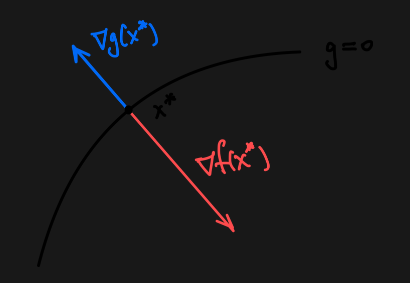
\includegraphics[width=0.4\textwidth]{Figs/kkt.png}
\caption{Graphical interpretation of KKT conditions on a single constraint.}
\label{fig:kkt}
\end{figure}


\subsection{Benefits of the Dual Problem}

The dual problem can be advantageous because it may be easier to solve than the primal problem. Additionally, it offers insights into the sensitivity of the optimal value to changes in the objective function or constraints. The duality gap, the difference between the solutions of the primal and dual problems, is zero under certain conditions, which provides a certificate of optimality for the primal solution.

%
%
%

\section{Smooth functions}
\subsection{Definition by derivatives}
\subsection{Definition by coefficients of Fourier transform}

\section{Singular value decomposition (SVD)}
\subsection{Definition}
\subsection{Properties}
\subsection{Applications}

%
%
%
%
%
%
%
%
%
%
%
%
%
%
%
%

\chapter{The Point Neuron}

\section{A Learning system}
\subsection{Supervised vs unsupervised learning vs reinforcement learning}

%
%
%

\subsection{Basic concepts in learning theory}

%
%
%

\subsection{The challenge of learning}
\subsubsection{Trainability}
The learning system's ability to arrive at the correct solution.

\subsubsection{Expressibility (capacity)}
The learning system's ability to represent complex functions.
We can choose the model for a given problem some examples are:
\begin{itemize}
    \item Linear regression $y = \mathbf{w}^T \mathbf{x} = b$
    \item Quadratic regression $y = \mathbf{w_2} \lVert \mathbf{x} \rVert^2 + \mathbf{w_1} \mathbf{x} + \mathbf{w_0}$
    \item Polynomial regression $y = \sum_{i=0}^{N} \mathbf{w_i} \lVert \mathbf{x} \rVert^i$
            While the equation is non linear in the input, it is quadratic in the weights, so the error function is convex.

    \item Fourier series $y = \sum_{k=n}^{N} \mathbf{w_k} e^{i k \pi \mathbf{x} / P}$ 
\end{itemize}
Using reacher models we can represent more complex functions, but we need to be careful with overfitting.

\subsubsection{Generalization}

\begin{definition}[Training error]
$E_{tr} = \frac{1}{P} \sum_{\mu=1}^{P} (\hat{y}(\mathbf{x}^\mu, \mathbf{w}) - y^\mu)^2$
\end{definition}

\begin{definition}[Generalization error]
$E_{g} = \int P(\mathbf{x}) (\hat{y}(\mathbf{x}, \mathbf{w}) - y(\mathbf{x}))^2 d\mathbf{x}$
\end{definition}

We have 2 assumptions:
\begin{itemize}
    \item All input come from some distribution $x^\mu \sim P(x)$. In most applications we will assume that any sample from the training set is an independent and identically distributed (i.i.d.) sample from the distribution $P(x)$.
    \item There is an underlying pattern in the labels $y^\mu \sim P(y|x^\mu)$
\end{itemize}
We will always have $E_{tr} \leq E_{g}$.

\begin{figure}
    \centering
    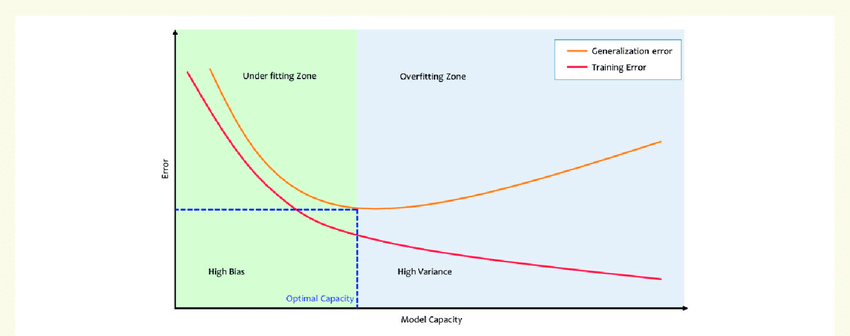
\includegraphics[width=\linewidth]{Figs/capacity-error-curve.png}
    \caption{Capacity VS Error curve}
    \label{fig:scenario1}
\end{figure}

\subsubsection{No free lunch theorem (NFT)}
\begin{theorem}
    If an algorithm performs well on a certain class of problems, it necessarily pays for that with degraded performance on the set of all remaining problems.
\end{theorem}
\begin{corollary}
    Every 2 optimization algorithms are equivalent when their performance is averaged across all possible problems.
\end{corollary}

\subsubsection{Regularization}
\begin{definition}
    Regularization is a technique used to prevent overfitting by discouraging overly complex models.
\end{definition}

\begin{itemize}
    \item Sparse parameters: $E_{tr}(\mathbf{w}) = \sum_{\mu=1}^{P} (\hat{y}(\mathbf{x}^\mu, \mathbf{w}) - y^\mu)^2 + \lambda \lVert \mathbf{w} \rVert_0$
    \item L1 regularization (Lasso): $E_{tr}(\mathbf{w}) = \sum_{\mu=1}^{P} (\hat{y}(\mathbf{x}^\mu, \mathbf{w}) - y^\mu)^2 + \lambda \lVert \mathbf{w} \rVert_1$
    \item L2 regularization: $E_{tr}(\mathbf{w}) = \sum_{\mu=1}^{P} (\hat{y}(\mathbf{x}^\mu, \mathbf{w}) - y^\mu)^2 + \lambda \lVert \mathbf{w} \rVert_2^2$
        We can solve this optimization problem analytically, and the solution is $\mathbf{w}^* = (\mathbf{X}\mathbf{X}^T + \lambda \mathbf{I})^{-1}\mathbf{X}\mathbf{Y}$
\end{itemize}


%
%
%

\section{Linear regression}
\subsection{Definition of the problem}
\begin{itemize}
    \item $\vec{x} \in \mathbb{R}^N$ - the input vector
    \item $y = \sum_{i=1}^{N} w_i x_i = \vec{w}^T \vec{x}$ - the output
    \item The training set: $\{(\vec{x}^1, y^1), (\vec{x}^2, y^2), \ldots, (\vec{x}^P, y^P)\} = \{(\vec{x}^\mu, y^\mu)\}_{\,\mu=1}^{P}$
    \item The training error of a single example (MSE): $\epsilon^\mu = (\hat{y}(\vec{x}^\mu, \vec{w}) - y^\mu)^2 = (\vec{w}^T \vec{x}^\mu - y^\mu)^2$
    \item The average error of a training set: $E_{tr}(\vec{w}) = \frac{1}{P} \sum_{\mu=1}^{P} \epsilon^\mu = \frac{1}{P} \sum_{\mu=1}^{P} (\vec{w}^T \vec{x}^\mu - y^\mu)^2$
    \item The generalization error: $E_{g}(\vec{w}) = \int P(\vec{x}) (\vec{w}^T \vec{x} - y(\vec{x}))^2 d\vec{x}$
\end{itemize}

%
%

\subsection{Points in general position}
\begin{definition}
A set of points in \(\mathbb{R}^n\) is said to be in \textit{general position} if no subset of \(m+1\) points lies in any \(m\)-dimensional hyperplane, for any \(m < n\). In simpler terms, in \(\mathbb{R}^2\) (the plane), points in general position means that no three points are collinear. Similarly, in \(\mathbb{R}^3\), no four points lie on the same plane. This concept extends to higher dimensions accordingly.
\end{definition}

%
%

\subsection{The optimal solution}

We will define the (empirical) feature covariance matrix of the input as:
\begin{align*}
    \mathbf{C_{tr}} = \frac{1}{P} \sum_{\mu=1}^{P} \vec{x}^\mu (\vec{x}^\mu)^T \\
    (\mathbf{C_{tr}})_{ij} = \frac{1}{P} \sum_{\mu=1}^{P} x_i^\mu x_j^\mu
\end{align*}

We will define the input-output covariance vector as:
\begin{align*}
    \vec{U_{tr}} = \frac{1}{P} \sum_{\mu=1}^{P} y^\mu \vec{x}^\mu \\
    (\vec{U_{tr}})_i = \frac{1}{P} \sum_{\mu=1}^{P} y^\mu x_i^\mu
\end{align*}

The weights that achieve the minimal loss must satisfy $\nabla E_{tr}(\vec{w}) = 0$. 
\begin{align*}
    \nabla \left(\frac{1}{P} \sum_{\mu=1}^{P} (\vec{w}^T \vec{x}^\mu - y^\mu)^2\right) = 0 \quad \\
    \Rightarrow \quad \frac{1}{P} \sum_{\mu=1}^{P} 2(\vec{w}^T \vec{x}^\mu - y^\mu) \vec{x}^\mu = 0 \\ 
    \Rightarrow \frac{1}{P} \sum_{\mu=1}^{P} (\vec{w}^T \vec{x}^\mu) \cdot \vec{x}^\mu  - \frac{1}{P} \sum_{\mu=1}^{P} y^\mu \vec{x}^\mu = 0 \\
    \Rightarrow \frac{1}{P} \sum_{\mu=1}^{P} \vec{x}^\mu (\vec{x}^\mu)^T \vec{w}  - \frac{1}{P} \sum_{\mu=1}^{P} y^\mu \vec{x}^\mu = 0 \\
    \Rightarrow \mathbf{C_{tr}} \vec{w} - \vec{U_{tr}} = 0 \\
\end{align*}

Alternatively, in vectorized notation:
\begin{align*}
    \mathbf{X} &= (\vec{\mathbf{x}}_1, \vec{\mathbf{x}}_2, \ldots, \vec{\mathbf{x}}_P) \in \mathbb{R}^{N \times P}, \quad
    \tilde{\mathbf{y}} = (y_1, y_2, \ldots, y_P) \in \mathbb{R}^P \\
    \nabla_{\mathbf{w}} E_{\text{tr}} (\mathbf{w}) &= 0 \\
    \frac{1}{P} \nabla_{\mathbf{w}} \lVert \mathbf{X}^T\mathbf{w} - \vec{\mathbf{y}} \rVert^2 &= 0 \\
    \nabla_{\mathbf{w}} (\mathbf{X}^T\mathbf{w} - \vec{\mathbf{y}})^T (\mathbf{X}^T\mathbf{w} - \vec{\mathbf{y}}) &= 0 \\
    \nabla_{\mathbf{w}} (\mathbf{w}^T\mathbf{X}\mathbf{X}^T\mathbf{w} + \vec{\mathbf{y}}^T\vec{\mathbf{y}} - 2\mathbf{w}^T\mathbf{X}\mathbf{Y}) &= 0 \\
    2\mathbf{X}\mathbf{X}^T\mathbf{w} - 2\mathbf{X}\mathbf{Y} &= 0 \\
\end{align*}

\subsubsection{The solution for P $\geq$ N}

\begin{theorem}
    The matrix \(\mathbf{C_{tr}}\) is positive definite if the input vectors are in general position and \(P \geq N\).
\end{theorem}

\begin{proof}
    \begin{align*}
        \mathbf{C_{tr}} &= \frac{1}{P} \sum_{\mu=1}^{P} \vec{x}^\mu (\vec{x}^\mu)^T \\
        \vec{v}^T \mathbf{C_{tr}} \vec{v} &= \frac{1}{P} \sum_{\mu=1}^{P} \vec{v}^T \vec{x}^\mu (\vec{x}^\mu)^T \vec{v} \\
        &= \frac{1}{P} \sum_{\mu=1}^{P} (\vec{v}^T \vec{x}^\mu) (\vec{v}^T \vec{x}^\mu)^T \\
        &= \frac{1}{P} \sum_{\mu=1}^{P} \lVert \vec{v}^T \vec{x}^\mu \rVert^2 \geq 0
    \end{align*}
\end{proof}

\begin{theorem}
    The optimal weights that minimize the training error are given by:
    \begin{align*}
        \mathbf{w}^* &= (\mathbf{X}\mathbf{X}^T)^{-1}\mathbf{X}\mathbf{Y} = \mathbf{C_{tr}}^{-1}\mathbf{U_{tr}}
    \end{align*}
\end{theorem}


%

\subsubsection{The solution for P $<$ N}

\textcolor{red}{TODO}

%
%

\subsection{Learning with noisy teacher}

\textcolor{red}{The teacher provides noisy labels to the training set. The noise is modeled as a Gaussian distribution with zero mean and variance $\sigma^2$. The training error is now given by:}

%
%
%


\section{The point neuron}
\subsection{The neuron model}
\subsection{The binary perceptron}
\subsection{The perceptron learning algorithm}
\subsection{Geometrical interpretation on the learning}
\subsection{Cover's theorem (no proof)}

%
%
%


\section{SVM}
\subsection{The margin}
\subsection{Uniqueness of the solution}
\subsection{The SVM optimization problem}
\subsubsection{The primal problem}
\subsubsection{The dual problem}
\subsection{Dot product solution}
\subsection{Soft-margin SVM}

%
%
%
%
%
%
%
%
%
%
%
%
%
%
%
%


\chapter{A Single Layer}

\section{The Kernel Method}
\subsection{The dot product solution of the SVM}
\subsection{The XOR problem}
\subsection{Nonlinear decision boundaries}
\subsection{The kernel trick}
\subsection{Mercer's theorem}
\subsection{Common kernels}
\subsubsection{Polynomial kernel}
\subsubsection{Gaussian kernel}
\subsubsection{Sigmoid kernel}
\subsubsection{Admissible kernels}

\section{The Cerebellum}

\subsection{Cerebellar anatomy, physiology, and function}
The cerebellum accounts for approximately 10\% of the brain's volume but contains over 50\% of its neurons. It is known for its organized, preserved hierarchical feedforward structure. Traditionally associated with motor control and coordination, recent studies have linked the cerebellum to a variety of cognitive functions, including spatial reasoning, timing, language, and working memory.

\subsubsection{Basic facts}
The cerebellum is significant not only due to its volume but also due to the sheer number of neurons it contains. Its structure has been preserved across species, which indicates its importance in brain function.

\subsubsection{The cerebellum's function}
Historically, the cerebellum's function has been recognized as crucial for motor control. The classical view is that it fine-tunes motor control and coordination, interacting with the motor cortex and the motor system. The modern view extends its functions to interaction with various cortical areas, contributing to cognitive abilities.

\subsubsection{The cerebellum's anatomy}
The cerebellum's circuit includes parallel fibers, stellate and basket cells, Golgi cells, Purkinje cells, granule cells, climbing fibers, mossy fibers, and the Deep Cerebellar Nuclei. Each of these components plays a specific role in cerebellar processing.

\subsubsection{The cerebellar circuit}
Inputs to the cerebellum come through mossy fibers and a single climbing fiber, while the output is mediated by the Purkinje cells. An error signal is thought to be provided by the climbing fibers.

\begin{figure}[ht]
    \centering
    \begin{subfigure}[b]{0.5\textwidth}
        \centering
        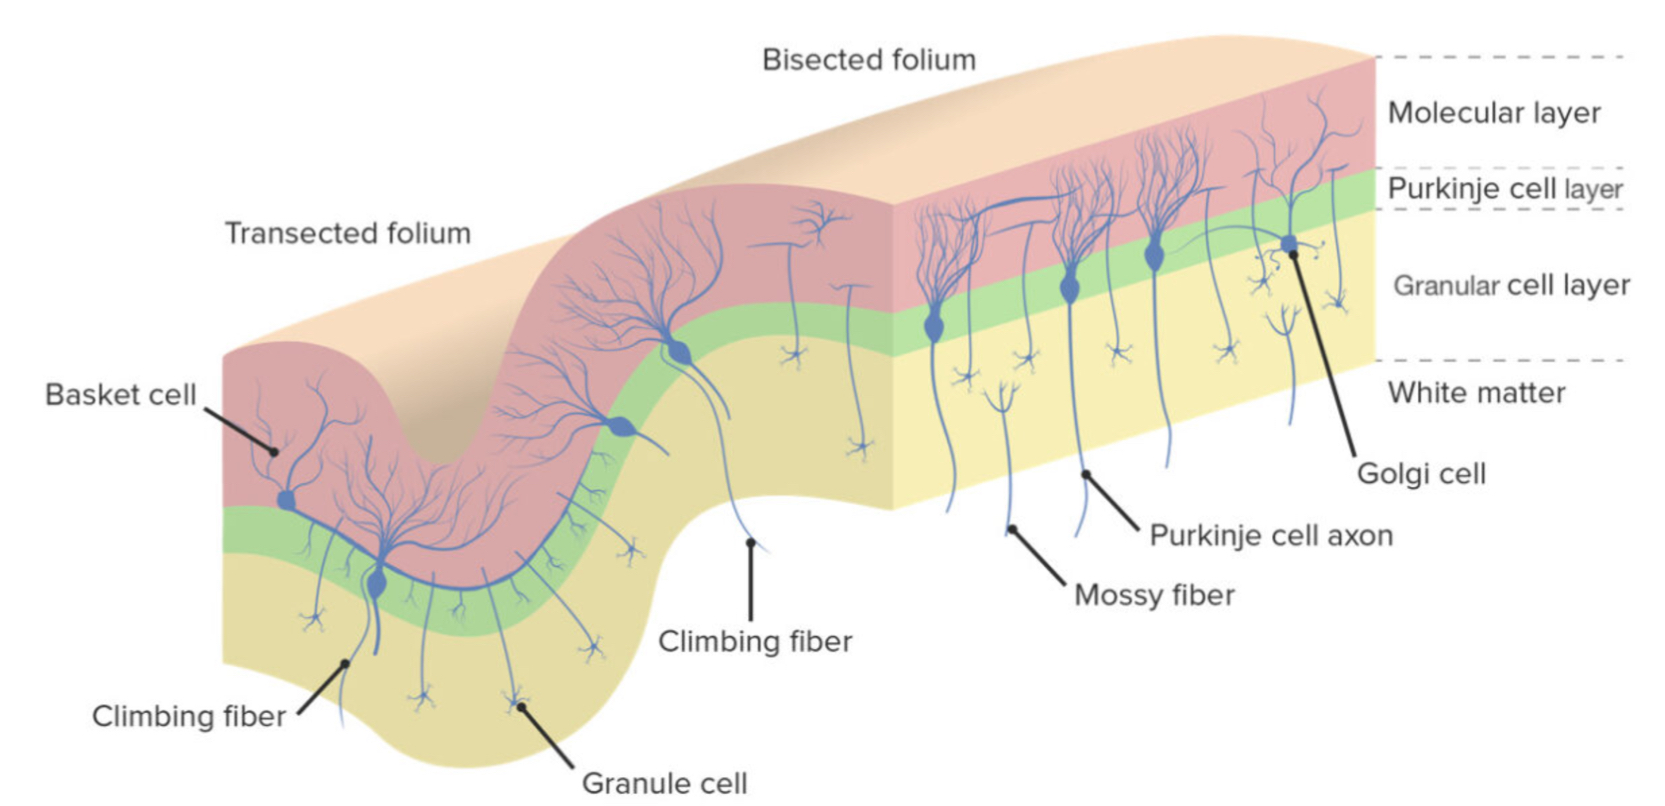
\includegraphics[width=\textwidth]{./Figs/cerebellums_anatomy.jpg}
        \label{fig:first_subfig}
    \end{subfigure}
    \hfill
    \begin{subfigure}[b]{0.5\textwidth}
        \centering
        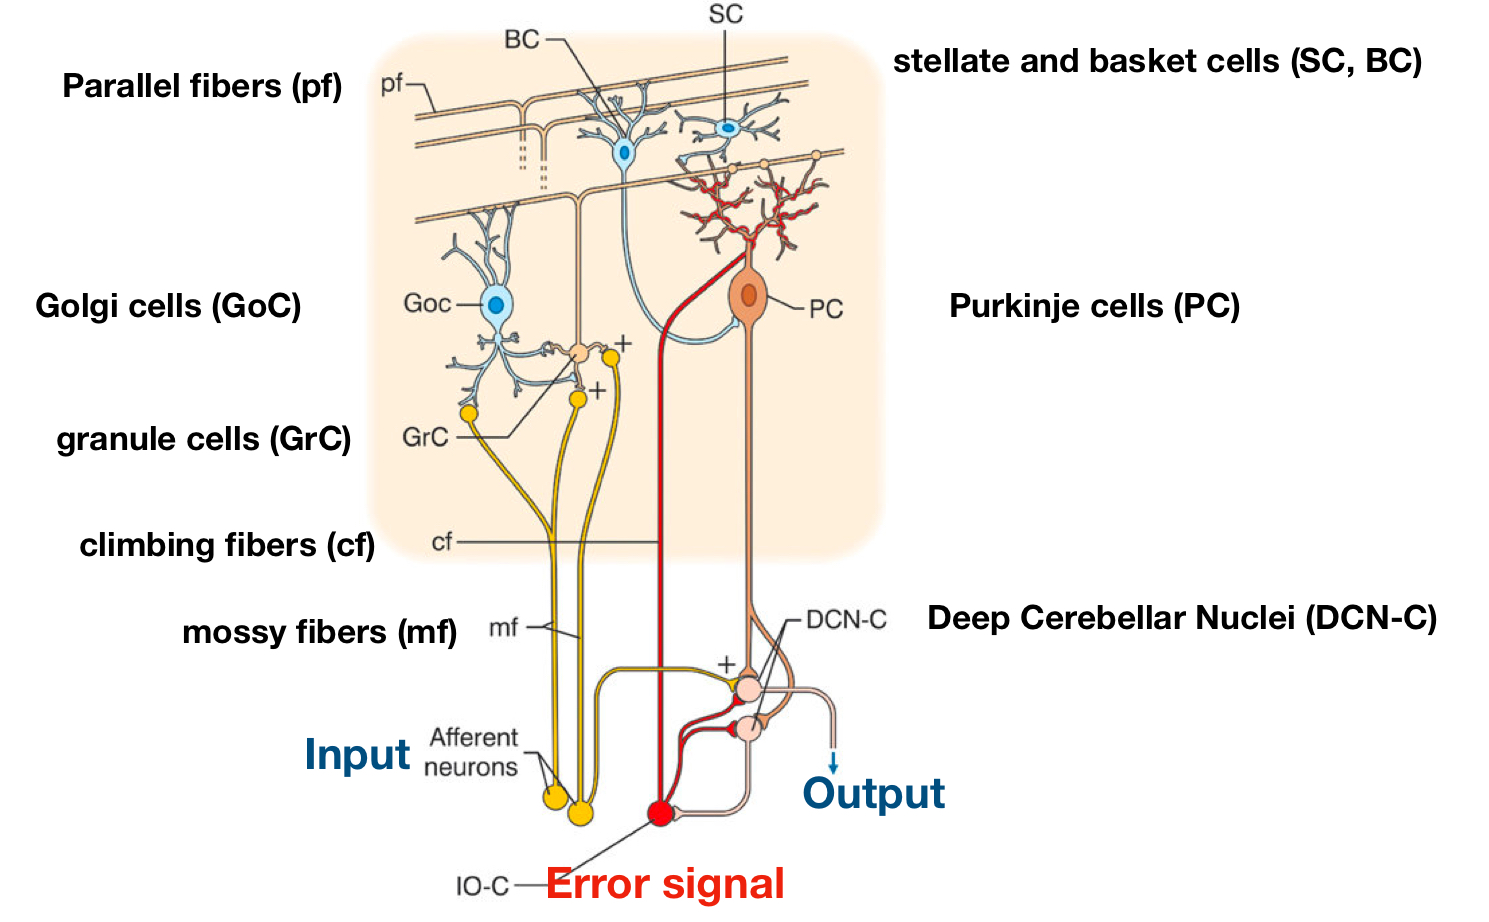
\includegraphics[width=\textwidth]{./Figs/cerebellums_anatomy2.jpeg}
        \label{fig:second_subfig}
    \end{subfigure}
    \hfill
    \begin{subfigure}[b]{0.5\textwidth}
        \centering
        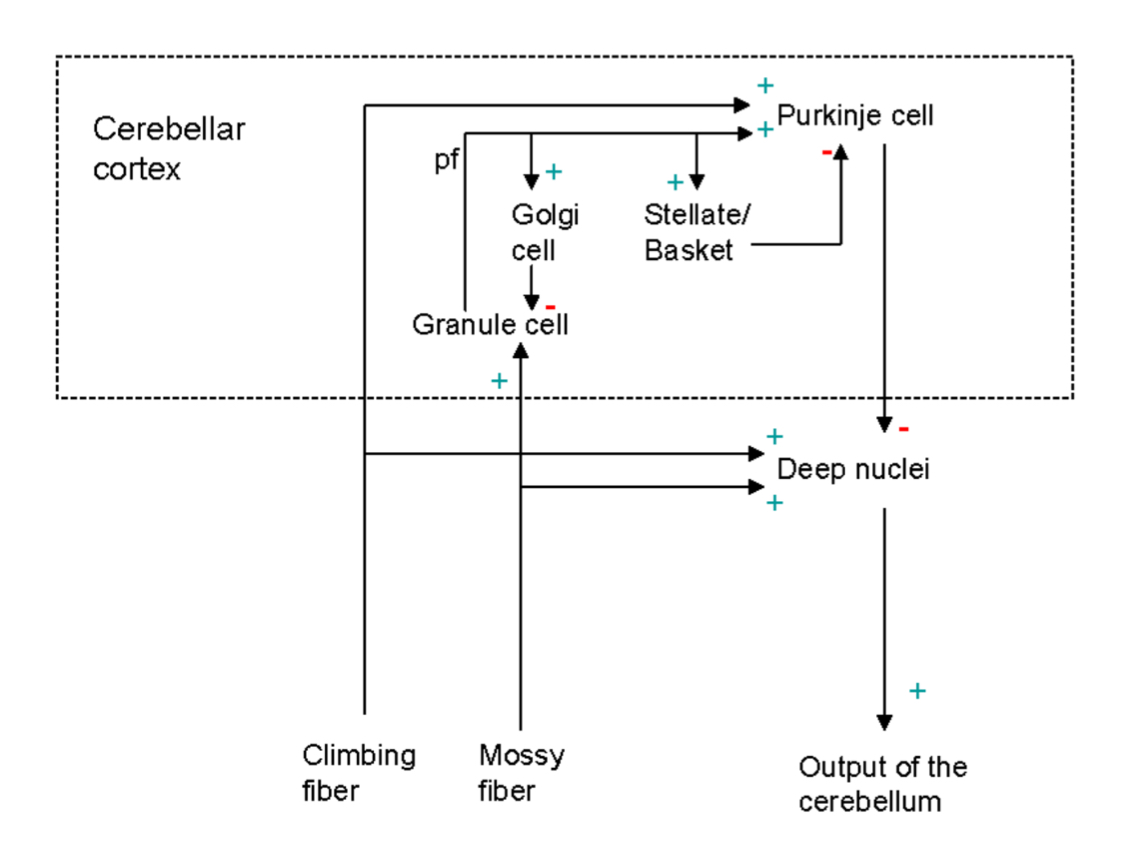
\includegraphics[width=\textwidth]{./Figs/cerebellums_anatomy3.jpeg}
        \label{fig:third_subfig}
    \end{subfigure}
    \label{fig:three_subfigures}
    \caption[short]{The cerebellum's anatomy.}
\end{figure}


\subsubsection{The cerebellar computational unit}
The computational unit of the cerebellum includes inputs from ~1,000 mossy fibers and a single climbing fiber, which are processed by ~200,000 parallel 
fibers and inhibitory interneurons, eventually influencing the output through a single Purkinje cell.

\subsubsection{Divergence and convergence in the cerebellum}
The cerebellum demonstrates a remarkable level of divergence and convergence. For instance, approximately 200 million mossy fibers diverge into 40 billion granule cells and then converge onto 15 million Purkinje cells. This massive divergence and convergence is crucial for the cerebellum's computational capacity.

\subsection{Plasticity and learning in the cerebellum}

\subsubsection{The Purkinje cell}
The Purkinje cell is unique for its planar dendritic arbor and is the sole output of the cerebellar cortex, inhibiting the Deep Cerebellar Nuclei. The plasticity observed in Purkinje cells is a central mechanism for cerebellar learning.
The Purkinje cell responds to climbing fiber inputs with a massive, all-or-none, 'complex spike'. The comlex spikes are relattively rare. 

\begin{figure}[ht]
\centering
\centering
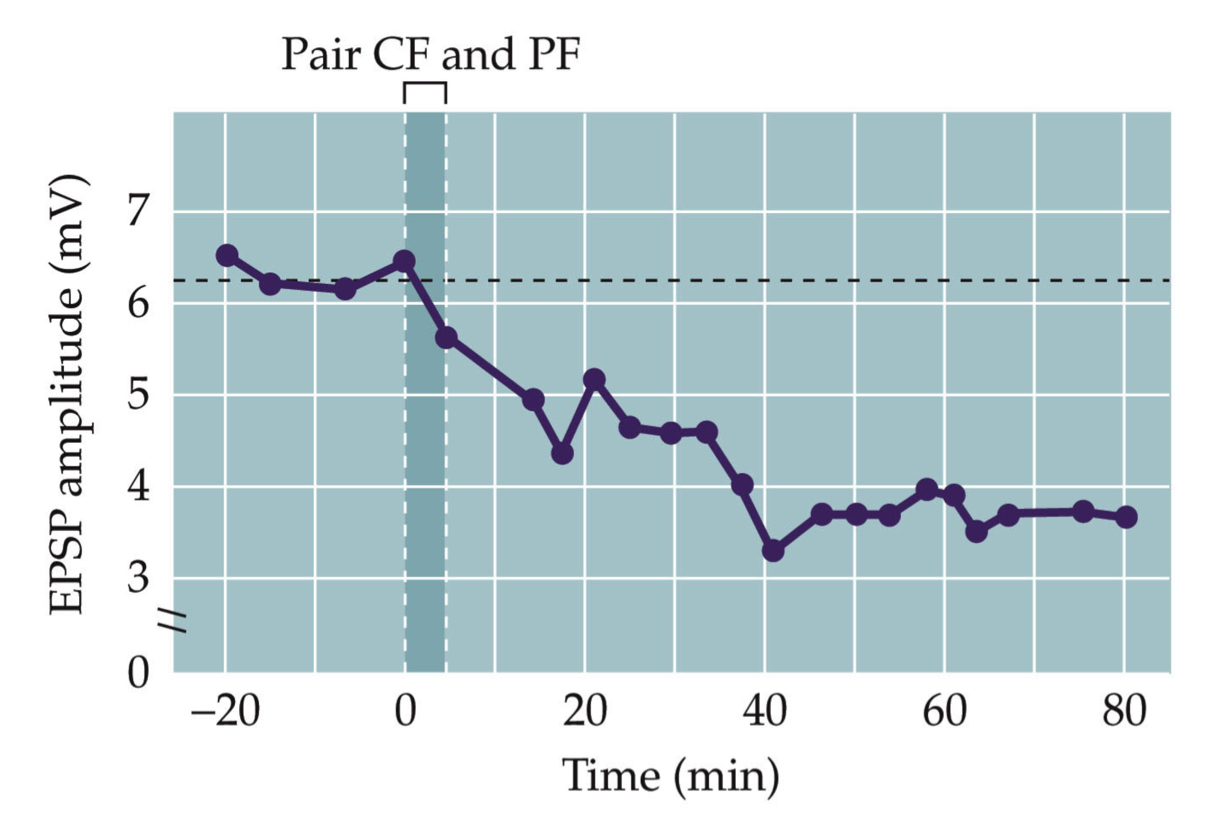
\includegraphics[width=0.6\textwidth]{./Figs/CF_PF.jpeg}
\label{fig:CF_PF}
\caption{When both CF (Climbing Fiber) and PF (Parallel Fiber) are active, LTD is induced.}
\end{figure}

\subsubsection{LTD and LTP in the Purkinje cell}
Long-Term Depression (LTD) and Long-Term Potentiation (LTP) in the Purkinje cells are responses to the synaptic activity between parallel fibers and climbing fibers. Climbing fibers signal errors, leading to LTD when paired with parallel fiber activation, and LTP occurs when parallel fibers are activated without climbing fibers.

\subsection{Marr-Albus theory for learning in the cerebellum}

\subsubsection{Motor learning in the cerebellum}
The Marr-Albus theory posits that the mossy fibers provide input patterns while the inferior olive generates an error signal when unexpected sensory input occurs. This framework helps explain how the cerebellum adapts and learns from motor errors, with the Purkinje cells playing a pivotal role.

\subsubsection{Main points the theory explains}
The theory explains the low frequency of complex spikes and climbing fiber firing, suggesting that these fibers do not contribute to ongoing motor execution but instead provide error signals for motor learning and adaptation.

\subsubsection{Extensions to the perceptron theory}
Recent studies have extended the perceptron theory, indicating that while the expansion of inputs helps, the benefits are limited without specific structural organization. Additionally, more layers in the cerebellar network model can lead to better learning outcomes.

\section{Gradient-based Learning}
\subsection{Batch learning}
\subsection{Stochastic gradient descent (SGD)}
\subsection{Online learning}
\subsubsection{Analysis of online learning dynamics}
\subsubsection{Dynamics of learning in a linear network}
\subsubsection{Dynamics of the average}
\subsubsection{Controlling the variance (learning rate)}


%
%
%
%
%
%
%
%
%
%
%
%
%
%
%
%


\chapter{Deep Neural Networks}

\section{Multi-layered perceptrons vs the kernel method}
The differences between the kernel method and multi-layered perceptrons:
\begin{itemize}
    \item In MLP the is no expansion. We only relied on the non-linearity of the activation function.
    \item All the weights need to be learned to solve the problem. In the kernel method, we only need to learn the support vectors. 
    The feature space was used to untie the non-linearity of the problem.
    \item The benefits of the kernel method are:
    \begin{itemize}
        \item Better performance in high dimensional spaces.
        \item No need to engineer the features.
        \item In online learning (the kernel method used all the data to learn the support vectors).
        \item Complexity with very large data sets-like the ones required for many modern applications.
    \end{itemize}
\end{itemize}

\section{Structure}
\begin{itemize}
    \item The architecture consists of $L$ layers.
        Each layer $l$ has $N_l$ neurons, where $l = 1, 2, \ldots, L$.
        The first layer contains $N_0$ neurons, which is the dimensionality of the input.
        The $L-1$ hidden layers can contain any number of neurons.
        The last layer contains $N_L$ neurons, which is the dimensionality of the output and is determined by the problem.
        \begin{itemize}
            \item It can be any activation function for regression problems.
            \item For binary classification, the output can be binary.
            \item For multi-class classification, the output can be a softmax function, which has the following formula:
            $\hat{y_i} (s_i^L) = \frac{e^{s_i^L}}{\sum_{j=1}^{N_L} e^{s_j^L}} , \mathbb{R} \rightarrow (0, 1)$
            Here the readout neurons are no longer independent, and the output is normalized to sum to 1. 
            The outputs represent the probability of the input belonging to each class.
        \end{itemize}
    \item Denote by $\phi$ the non-linear activation function, by $W^l$ the matrix $N_l \times N_{l-1}$ of weights, that leads from $s^{l-1}$ to $s^l$. 
        The output of the $l$-th layer is given by 
        \begin{align*}
            s^l = \phi(W^l s^{l-1}) \\
            s_i^l = \phi(\sum_{j=1}^{N_{l-1}} W_{ij}^l s_j^{l-1}) = \phi((w_i^l)^T s^{l-1}) \\ 
            s^0 = x , N_0 = N, s^L = y
        \end{align*}
\end{itemize}

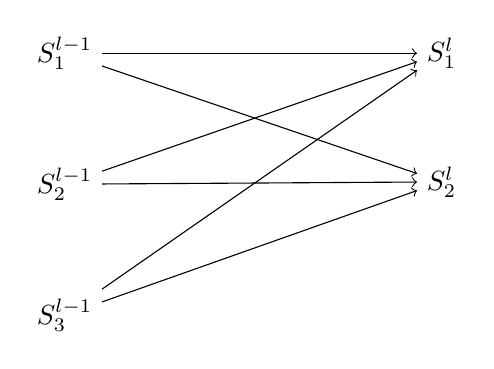
\begin{tikzpicture}[node distance=1cm and 2cm]
    % Define nodes
    \node (s1) {\( S_1^{l-1} \)};
    \node[below=of s1] (s2) {\( S_2^{l-1} \)};
    \node[below=of s2] (s3) {\( S_3^{l-1} \)};
    \node[right=of s1, xshift=2cm] (s4) {\( S_1^{l} \)};
    \node[below=of s4] (s5) {\( S_2^{l} \)};
    % Connect nodes
    \foreach \i in {1,...,3}
        \foreach \j in {4,...,5}
            \draw[->] (s\i) -- (s\j);
\end{tikzpicture}
\begin{tikzpicture}
    % Draw matrix
    \node[right=of s2, xshift=1cm] (matrix) {
        \( W^l = \begin{pmatrix}
            w_{11} & w_{12} & w_{13} \\
            w_{21} & w_{22} & w_{23}
        \end{pmatrix} \)
    };
    % Draw equation
    \node[right=of s5, xshift=2cm] (equation) {
        \( S^l = \phi(W^l S^{l-1}) \)
    };
\end{tikzpicture}

\subsection{Activation functions}
Typical activation functions include:
\begin{itemize}
    \item The sigmoid function (logistic) : $\phi(x) = \frac{1}{1 + e^{-x}}, \mathbb{R} \rightarrow (0, 1)$
    \item The hyperbolic tangent function: $\phi(x) = \tanh(x) , \mathbb{R} \rightarrow (-1, 1)$
    \item The rectified linear unit (ReLU): $\phi(x) = \max(0, x) , \mathbb{R} \rightarrow [0, \infty)$
    \item The leaky ReLU: $\phi(x) = \max(\alpha x, x), \alpha \in (0, 1), \mathbb{R} \rightarrow (-\infty, \infty)$
\end{itemize}

\begin{figure}
    \centering
    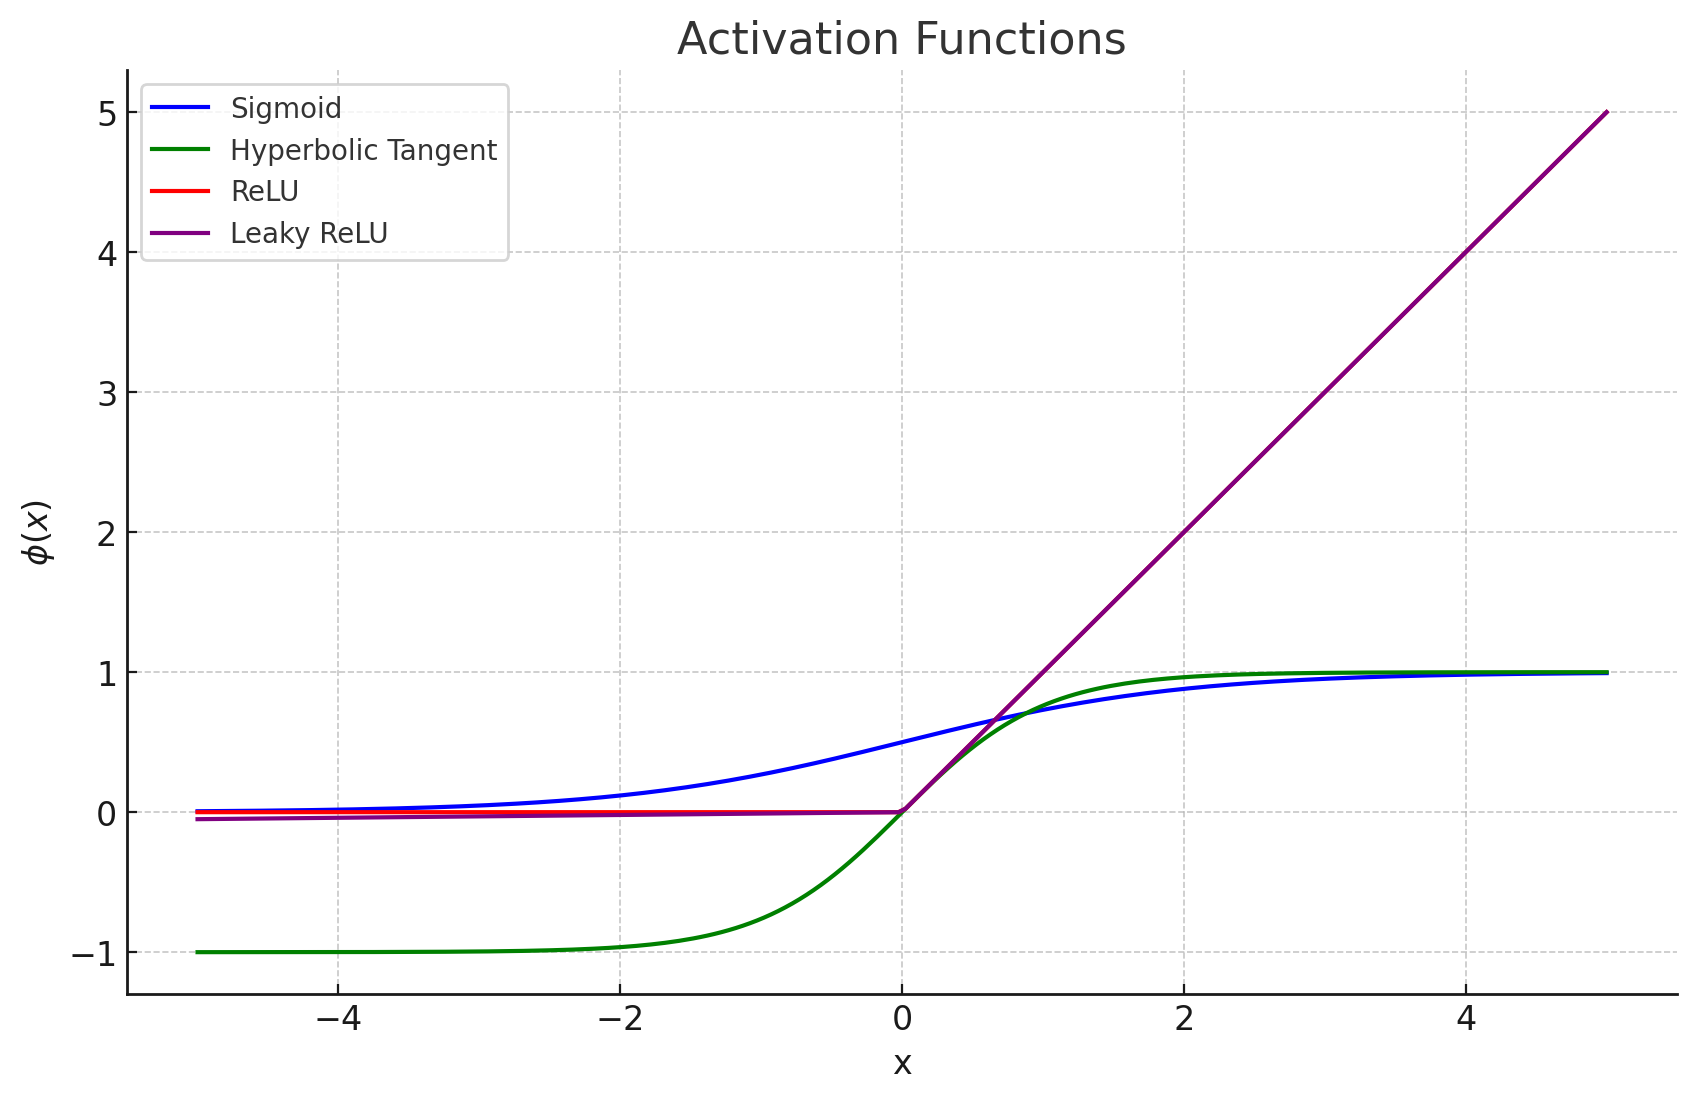
\includegraphics[width=0.6\linewidth]{Figs/activation_functions.png}
    \caption{Activation functions}
\label{fig:activation_functions}
\end{figure}


\subsection{Loss functions}
The quadratic loss function is given by:
\begin{align*}
    \epsilon(\mathbf{w}) = \frac{1}{2} \lVert \hat{\mathbf{y}}(\mathbf{x}, \mathbf{w}) - \mathbf{y} \rVert^2
\end{align*}
Algorithms may include regularization terms to prevent overfitting, such as the L1 and L2 regularization terms, and the optimization is over Lagrangian.

\subsection{Credit assignment and backpropagation}

\section{Backpropagation derived using Lagrange multipliers}

\section{Dynamics of learning in a linear network (no proof)}

\section{Shallow networks}
\subsection{Universal approximation theorem}
\subsection{Barron's theorem}
\subsection{The curse of dimensionality (Mhaskar)}

%
%
%

\section{Deep and shallow networks in the brain}

\section{Why go deep?}
\subsection{Expressivity}
\subsubsection{Size efficiency of deep networks}
\subsubsection{Exponential expressivity in deep networks}
\subsubsection{Manifold disentanglement}
\subsection{Trainability}
\subsubsection{Sample complexity}
\subsubsection{Training shallow vs deep networks}
\subsubsection{The importance of a good initialization}
\subsection{Generalization}
\subsubsection{The overparameterized regime}
\subsubsection{Why are deep networks good at generalization?}

\section{Visual processing in the brain}
\subsection{The visual pathway}
\subsection{The visual cortex}
\subsection{The receptive field}


%
%
%
%
%
%
%
%
%
%
%
%
%
%
%
%


\chapter{Recurrent Neural Networks}

\section{Circuit equations for RNNs}


\subsection{The dynamics of a single neuron in a discrete time}
Output of a neuron is given by:
\[
    s_i(t) = \phi(h_i(t))
\]
Point neuron (in time) is given by:
\[
    h_i(t + \bigtriangleup  t) = (1 - \bigtriangleup t) h_i(t) + \bigtriangleup t (\sum_{j=1}^N W_{ij} s_j(t) + u_ix(t))
\]
Where:
\begin{itemize}
    \item $h_i(t)$ is the membrane potential of the neuron $i$ at time $t$
    \item $s_i(t)$ is the output of the neuron $i$ at time $t$
    \item $\phi$ is the activation function
    \item $W_{ij}$ is the weight of the connection to neuron $i$ from neuron $j$
    \item $u_i$ is a vector of weights that connect the neuron to the external input
    \item $x(t)$ is the external input at time $t$
    \item $\bigtriangleup t$ is the time step
    \item $N$ is the total number of neurons in the network
\end{itemize}

\subsection{The dynamics of a RNN in a continuous time}
Consider a neural network with $N$ neurons with connectivity matrix $J \in \mathbb{R}^{N \times N}$, and external input $x(t) \in \mathbb{R}^N$.
The dynamics of the network are given by:
\[
    \frac{dh_i(t)}{dt} = -h_i(t) + \sum_{j=1}^N J_{ij} \phi(h_j(t)) + w_i^{in} I(t)
\]

and the output of the network is given by:
\[
    z(t) = \sum_{j=1}^N \nu_j \phi(h_j(t))
\]
Where:
\begin{itemize}
    \item $w_i$ is the input weights vector of the neuron $i$
    \item $h_j(t)$ is the membrane potential of the neuron $j$ at time $t$
    \item $\phi$ is the activation function
    \item $\nu_j$ is the readout weight of the neuron $j$
\end{itemize}

\begin{figure}
    \centering
    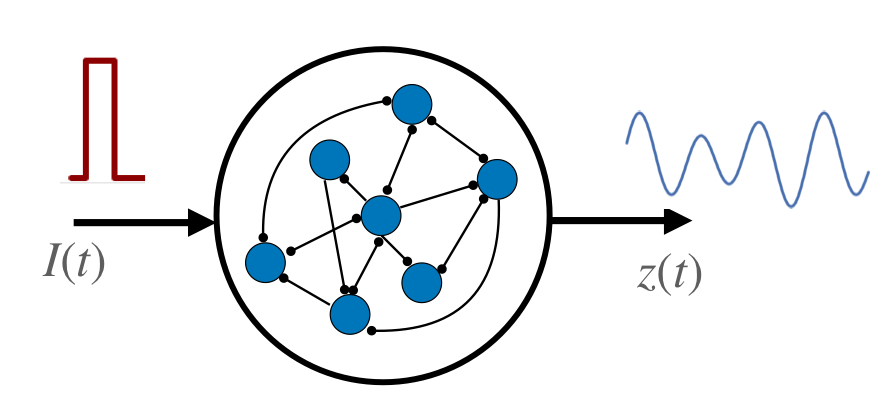
\includegraphics[width=0.6\textwidth]{Figs/RNN.jpeg}
    \caption{Recurrent Neural Network}
    \label{fig:rnn}
\end{figure}

\subsection{Examples of tasks solved with RNNs}

\section{Learning in RNNs}

Recurrent Neural Networks (RNNs) exhibit rich dynamics suitable for sequential data processing. 
Training RNNs, however, poses challenges due to the recurrent feedback of errors, amplifying them and complicating convergence, 
as well as making the credit assignment problem more difficult.

\subsection{Reservoir Computing}
In reservoir computing, the network is trained using the error of a linear readout of the units. 
This approach avoids the difficulties of training the entire network by only adjusting the readout weights.

\subsubsection{Open Circuit}
In an open circuit configuration, the network's output is not fed back during learning, preventing the amplification of initial errors. 
Instead, we make sure that we have the necessary ingredients to learn the output function by supplying the network with the desired output.
The dynamics of the network is given by:
\[
    \frac{dh_i(t)}{dt} = -h_i(t) + \sum_{j=1}^N J_{ij} \phi(h_j(t)) + w_i^{in} I(t) + u_i f(t)
\]
Once the network has been trained, we stop feeding it the target.
But without feeding the network with the target, the network is different from the one we trained.
Luckily, we have a good estimate of the output function $f(t) \approx z(t)$.

\begin{figure}[ht]
\centering
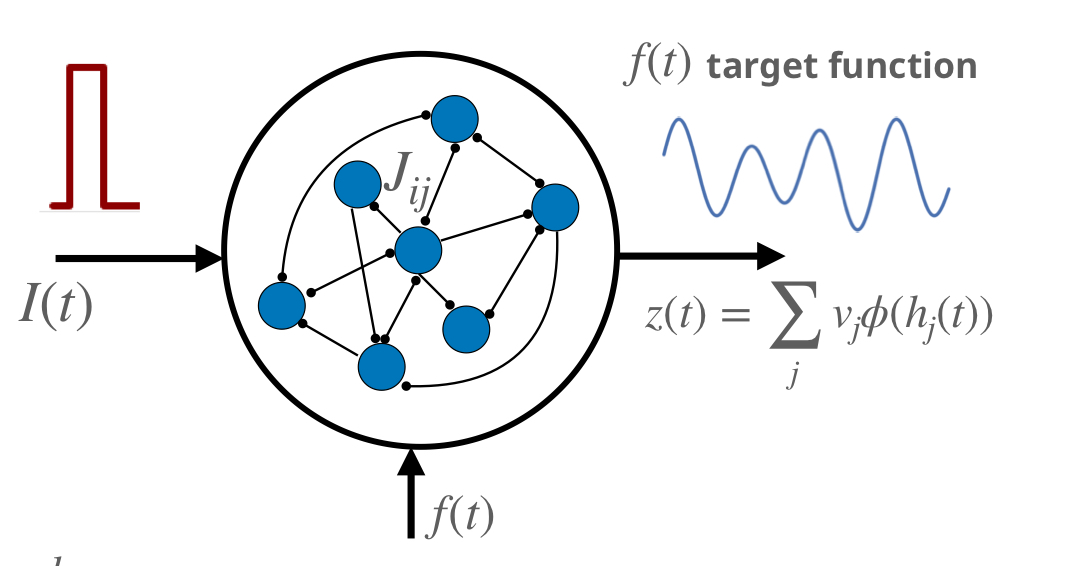
\includegraphics[width=0.6\textwidth]{Figs/RNN_open_circuit.jpeg}
\caption{Open circuit training of RNN.}
\label{fig:rnn_learning}
\end{figure}


\subsubsection{Closed Circuit (Echo/Liquid State Machines)}
In closed circuits, such as echo-state machines and liquid state machines, the output can be fed back into the network. 
If the network is trained properly, there is little to no difference from the open circuit.
The added solution is equivilent to a low-rank addition to $J_{ij}$.
The dynamics of the network is given by:
\begin{align*}
    \frac{dh_i(t)}{dt} = -h_i(t) + \sum_{j=1}^N J_{ij} \phi(h_j(t)) + w_i^{in} I(t) + u_i z(t) = \\
    -h_i(t) + \sum_{j=1}^N J_{ij} \phi(h_j(t)) + w_i^{in} I(t) + \sum_{j=1}^N u_i \nu_j \phi(h_j(t)) = \\
    -h_i(t) + \sum_{j=1}^N (J_{ij} + u_i \nu_j) \phi(h_j(t)) + w_i^{in} I(t) = \\
    -h_i(t) + \sum_{j=1}^N \tilde{J}_{ij} \phi(h_j(t)) + w_i^{in} I(t)
\end{align*}
Where: $\tilde{J}_{ij} = J_{ij} + u_i \nu_j$

\begin{figure}[ht]
\centering
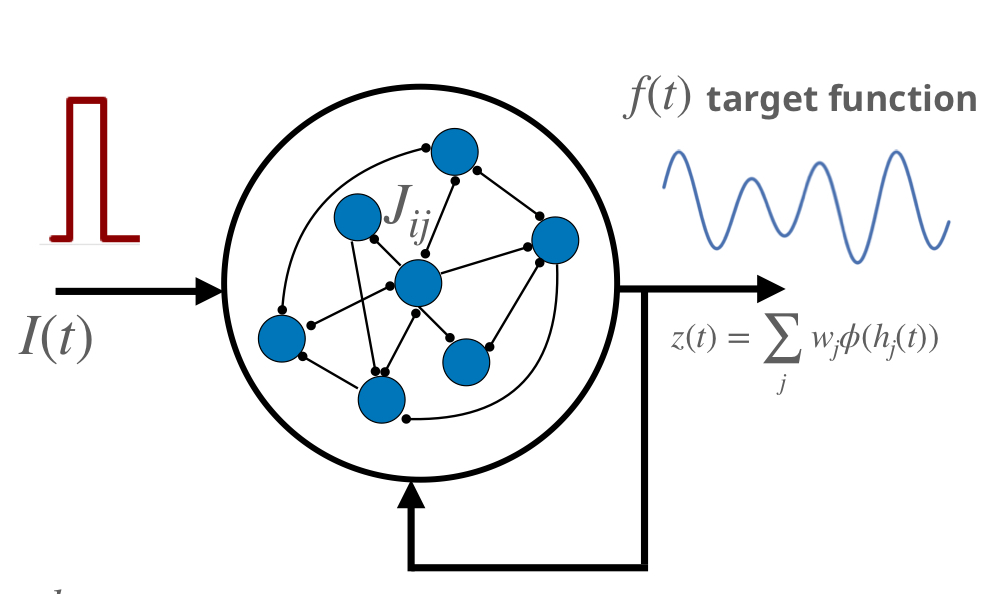
\includegraphics[width=0.6\textwidth]{Figs/RNN_closed_circuit.jpeg}
\caption{Closed circuit RNN.}
\label{fig:rnn_learning}
\end{figure}

\subsection{Recursive Least Squares (RLS)}
Recursive Least Squares (RLS) is a fast algorithm for linear regression over sequential data, 
minimizing a weighted linear least squares cost function. 
It is particularly well-suited for scenarios where parameters must be rapidly adjusted in response to evolving data streams.

\subsection{FORCE Learning (RLS on the Output Function)}
FORCE (First-Order Reduced and Controlled Error) learning is a closed-circuit training method for RNNs. 
In this approach, the output of the network can be fed back as input during the training process. 
Unlike open-circuit models, which do not feed the output back into the network during training,
FORCE learning leverages the feedback to adjust the synaptic weights quickly and effectively, reducing the magnitude of the output error. 

\subsubsection{Derivation}
RLS for FORCE learning is derived by minimizing a regularized weighted least squares cost function that accounts for the error at each time step 
and incorporates a discounting factor for older signals.
Consider an RNN with a readout that is defined at time t for every $t' < t$ as:
\[
    z(t') = \vec{w}(t) \cdot \vec{\phi} (h(t'))
\]
Given a sequence of signals $\{\vec{x}\}^t \subset \mathbb{R}^N$ we aim to learn weights $\vec{w}^*(t)$ that best approximate some target $f(t) = f(\{\vec{x}\}^t)$.
The error at time t' is given by:
\[
    \epsilon(t') = f(t') - z(t')
\]
We will define the weighted least squares cost function as:
\[
    L(\vec{w}(t)) = \sum_{t'=1}^t \lambda^{t-t'} \epsilon^2(t') + \alpha \lambda^t \lVert \vec{w}(t) \rVert^2
\]
Where:
\begin{itemize}
    \item $0 < \lambda \leq 1$ is the discounting factor
    \item $\alpha$ is the regularization parameter
\end{itemize}

The minimum of L w.r.t $\vec{w}(t)$ is given by:

\begin{align*}
   &0 = \frac{\partial L}{\partial {w_i}} = 2 \sum_{t'=1}^t \lambda^{t-t'} \epsilon(t') \frac{\partial \epsilon(t')}{\partial w_i} + 2 \alpha \lambda^t {w_i}(t) \\
   &(
        \frac{\partial \epsilon(t')}{\partial {w_i}} = 
        \frac{\partial f(t')}{\partial {w_i}} - \frac{\partial z(t')}{\partial {w_i}} =
        - \frac{\partial z(t')}{\partial {w_i}} =
        - \phi_i (t')
    ) \\
   &0 = - \sum_{t'=1}^t \lambda^{t-t'} \epsilon(t') \phi_i(t') + \alpha \lambda^t w_i(t) \\
   &0 = - \sum_{t'=1}^t \lambda^{t-t'} (f(t') - z(t')) \phi_i(t') + \alpha \lambda^t w_i(t) \\
   &0 = - \sum_{t'=1}^t \lambda^{t-t'} (f(t') - \vec{w}(t) \cdot \vec{\phi}(t')) \phi_i(t') + \alpha \lambda^t w_i(t) \\
   &0 = - \sum_{t'=1}^t \lambda^{t-t'} f(t') \phi_i(t') + \sum_{t'=1}^t \lambda^{t-t'} \sum_{j=1}^N w_j(t) \phi_j(t') \phi_i(t') + \alpha \lambda^t w_i(t) \\
   &\sum_{t'=1}^t \lambda^{t-t'} f(t') \phi_i(t') = \sum_{j=1}^N  \left[ \sum_{t'=1}^t \lambda^{t-t'} \phi_j(t') \phi_i(t') + \alpha \lambda^t \delta_{ij} \right] w_j^*(t) \\
   &(M_{ij}(t) \stackrel{\text{def}}{=}   \sum_{t'=1}^t \lambda^{t-t'} \phi_j(t') \phi_i(t') + \alpha \lambda^t \delta_{ij}
   & {u_i}(t) \stackrel{\text{def}}{=}   \sum _{t'=1}^t \lambda^{t-t'} f(t') \phi_i(t')) \\
   &\sum _{j=1}^N M_{ij}(t) w_j^*(t) = u_i(t) \\
   &M(t) \vec{w}^* = \vec{u}(t) \rightarrow \vec{w}^* = (M(t))^{-1} \vec{u}(t)
\end{align*}

This approach entails inverting the matrix M numerically every time step, which can be computationally expensive.

\subsubsection{Recursive Form of the Accumulative Covariance Matrix}
The accumulative covariance matrix, essential for updating the weights in RLS, can be computed recursively, allowing for efficient updates as new data arrives.
In the recursive form, the accumulative covariance matrix is given by:
\begin{align*}
    M_{ij}(t) = \sum_{t'=1}^t \lambda^{t-t'} \phi_i(t') \phi_j(t') =  \sum_{t'=1}^{t-1} \lambda^{t-t'} \phi_i(t') \phi_j(t') + \phi_i(t) \phi_j(t) \\
    {u_i}(t) = \sum _{t'=1}^t \lambda^{t-t'} f(t') \phi_i(t') = \sum _{t'=1}^{t-1} \lambda^{t-t'} f(t') \phi_i(t') + f(t) \phi_i(t)
\end{align*}
In the matrix form, the recursive update rule for the accumulative covariance matrix is given by:
\begin{align*}
    M(t) = \lambda M(t-1) + \vec{\phi}(t) \vec{\phi}(t)^T \\
    \vec{u}(t) = \lambda \vec{u}(t-1) + f(t) \vec{\phi}(t)
\end{align*}

We will define $P(t) \stackrel{\text{def}}{=} M^{-1}(t)$ and we will have:
\begin{align*}
    M^{-1}(t) =  P(t) = \frac{1}{\lambda} \left[ P(t-1) - \frac{P(t-1) \vec{\phi}(t) \vec{\phi}(t)^T P(t-1)}{\lambda + \vec{\phi}(t)^T P(t-1) \vec{\phi}(t)} \right]
\end{align*}

\subsubsection{Weights Update Rule}
The weights in FORCE learning are updated using a recursive delta rule that considers the current readout, the desired output, and the previously computed error to adjust the readout weights incrementally.

We will define the $\mathbf{gain-paramter} \quad \vec{k}(t)$ as 
\begin{align*}
    \vec{k}(t) \stackrel{\text{def}}{=} \frac{P(t-1) \vec{\phi}(t)}{\lambda + \vec{\phi}(t)^T P(t-1) \vec{\phi}(t)}
\end{align*}
and is holds that $\vec{k}(t) = P(t) \vec{\phi}(t)$, proof:
\begin{align*}
    &P(t) \vec{\phi}(t) = \frac{1}{\lambda} \left[ P(t-1) - \frac{P(t-1) \vec{\phi}(t) \vec{\phi}(t)^T P(t-1)}{\lambda + \vec{\phi}(t)^T P(t-1) \vec{\phi}(t)} \right] \vec{\phi}(t) \\
    &= \frac{1}{\lambda} \left[ P(t-1) \vec{\phi}(t) - \frac{P(t-1) \vec{\phi}(t) \vec{\phi}(t)^T P(t-1) \vec{\phi}(t)}{\lambda + \vec{\phi}(t)^T P(t-1) \vec{\phi}(t)} \right] \\
    &= \frac{1}{\lambda} \left[ \frac{\lambda P(t-1) \vec{\phi}(t) + P(t-1) \vec{\phi}(t) \vec{\phi}(t)^T P(t-1) \vec{\phi}(t) - P(t-1) \vec{\phi}(t) \vec{\phi}(t)^T P(t-1) \vec{\phi}(t) } {\lambda + \vec{\phi}(t)^T P(t-1) \vec{\phi}(t)} \right] = \\ 
    &= \frac{1}{\lambda} \left[ \frac{\lambda P(t-1) \vec{\phi}(t)}{\lambda + \vec{\phi}(t)^T P(t-1) \vec{\phi}(t)} \right] 
    = \frac{P(t-1) \vec{\phi}(t)}{\lambda + \vec{\phi}(t)^T P(t-1) \vec{\phi}(t)} = \vec{k}(t)
\end{align*}

The weights update rule is given by:
\begin{align*}
    \vec{w}^*(t) &= P(t) \vec{u}(t) \\
    &= P(t) \left[ \lambda \vec{u}(t-1) + f(t) \vec{\phi}(t) \right] \\
    &= \lambda P(t) \vec{u}(t-1) + f(t) \vec{k}(t) \\ 
    &= \left( P(t-1) - \frac{P(t-1) \vec{\phi}(t) \vec{\phi}(t)^T P(t-1)}{\lambda + \vec{\phi}(t)^T P(t-1) \vec{\phi}(t)} \right) \vec{u}(t-1) + f(t) \vec{k}(t) \\ 
    &= P(t-1) \vec{u}(t-1) - \vec{k}(t) \vec{\phi}(t)^T P(t-1) \vec{u}(t-1) + f(t) \vec{k}(t) \\
    &= \vec{w}^*(t-1) + k(t) \left[ f(t) - \vec{\phi}(t)^T \vec{w}^*(t-1) \right] \Longrightarrow \\
    \vec{w}^*(t) &= \vec{w}^*(t-1) + k(t) \left[ f(t) - \vec{\phi}(t)^T \vec{w}^*(t-1) \right] \\
    &= \vec{w}^*(t-1) + k(t) \left[ f(t) - z_{-} (t) \right]
\end{align*}

where $z_{-} (t) = \vec{\phi}(t)^T \vec{w}^*(t-1)$ is the predicted output at time $t$, before updating the weights.

If we consider the case where the case where $\vec{w}^{t+1} = \vec{w}^t + (f^t - z^t) P^t \vec{\phi}^t $, 
and the update rule for $P$ (the accumulative inverse correlation matrix) is given by $(P^{t+1})^{-1} = (P^t)^{-1}  + \vec{\phi}^t (\vec{\phi}^{t})^T$,
then the update rule for $P$ is given by:
\begin{align*}
    P^{t+1} = P^t - \frac{P^t \vec{\phi}^t (\vec{\phi}^t)^T P^t}{1 + (\vec{\phi}^t)^T P^t \vec{\phi}^t}
\end{align*}

%
%
%

\section{Cortical networks (motor cortex and prefrontal cortex)}
\subsection{Dynamic system hypothesis}
\subsection{Motor cortex untangles muscles trajectory}
\subsubsection{Supplementary motor area (SMA)}
\subsection{Context-dependent integration in prefrontal cortex}
\subsubsection{The prefrontal cortex}
\subsubsection{Key ideas}
\subsubsection{The experiment task, performance, and analysis}

%
%
%
%
%
%
%
%
%
%
%
%
%
%
%
%


\chapter{Reinforcement Learning}

\section{Definitions}
\subsection{Markov decision process (MDP)}
\subsection{Policy}
\subsection{Value function}
\subsection{Bellman equation}
\subsection{Bellman optimality}

\section{Pavlovian conditioning and the delta rule (Rescorla-Wagner)}

\section{Temporal difference learning (TD)}
\subsection{The TD error}
\subsection{The TD learning rule}

\section{Model-based methods}
\subsection{Dynamic programming}
\subsection{Value iteration}
\subsection{Policy iteration}


% Repeat the structure for chapters 2, 3, 4, and 5 following the provided structure

\backmatter
% Add any appendices or references here

\end{document}







        

